\section{Crawler}
In unsere Projekt wird ein Laufroboter verwendetder vom Labor für Intelligente Sensor-Aktuator-Systeme (ISAS) selbst aufgebaut wurde. Es bestehen viele verschiedene Versionen des Crawlers. Diese Roboter werden für mehrere Zwecke verwendet. Darüber hinaus ist das Chassis von diesen
Roboter komplett in 3D gedruckt. Daher können diese sehr schnell gebaut werden.


\begin{figure}[b!]
	\centering
	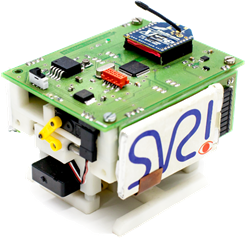
\includegraphics[width=0.5\linewidth]{Images/crawler}
	\caption{Der Crawler}
	\label{fig:crawler}
\end{figure}

\subsection{Aufbau}
Der Crawler, der im Projekt benutzt wird, ist die neueste Version. Die Hauptkomponente der Version ist ein Arduino Yun.
\\Der Arduino Yun verfügt über ein WLAN-Modul, mit dem ein WLAN generiert Oder in ein bestehendes WLAN eingefügt wird. Der Craeler verfügt es über drei verschiedene Beine, wobei jedes einzeln mittels Servomotor gesteuert werden kann. Dies ermöglicht dem Roboter, sich gerade, seitlich und omnidirektional zu bewegen.
\\Der Crawler enthält vier Ultraschallsensoren und eine IMU. Es sind insgesamt vier Ultraschallsensoren installiert, die jeweils aus einem bestehen Empfänger und ein Sender existieren.  Die Sensoren sind in 90-Winkeln zueinander angeordnet
\\Zusätzlich befinden sich oben zwei LEDs (gelb und rot), mit denen der
Roboter einfacher, zum Beispiel von einer Deckenkamera, verfolgt werden kann.
Das Design der Roboter ermöglicht eine Vielzahl unterschiedlicher Grundfunktionen Bewegungsmuster.










\subsection{Position- und Rotationschätzung mittels Kameratracking}
Zur bessere Simulation und Evaluierung muss die genau Position und Rotation ermittelt werden. Dazu wird ein Deckenkamerasystem verwendet. Zur Ermittelung der Position unseres Laufroboters wird ein rote LED auf dem Crawler aktiviert, die durch das an der Decke befestigte Kamerasystem aufgenommen wird. Durch eine Farberaum-Umwandlung kann die rote Markierung im Bild zuverlässig gefunden werden. Mittles anschließender  Koordinatentransform, die und Gleichung \ref{fig:coordinates} gezeigt ist,  wird die Position des echten Crawlers ermittelt und umgewandelt.
Für die Rotation wird entsprechend eine zweite gelbe LED in Crawler eingesetzt, durch den bekannten Aufbau kann die Bewegungsrichtung durch das Kamerasystem erkannt werden. Die gesammelten Bewegungsdaten können zusammen mit den Messdaten des Crawlers als Ground Truth exportiert werden. Das ganze Prozess wird durch unten stehend Bild dargestellt.

\begin{figure}
    \centering
    \left[ \begin{array}{c}
    x_{k+1} \\ 
    y_{k+1} \\ 
    \Phi_{k+1}
    \end{array} \right] =\left[ \begin{array}{c}
    x_{k} \\ 
    y_{k} \\ 
    \Phi_{k}
    \end{array} \right]+\left[ \begin{array}{ccc}
    cos(\Phi_{k}) & -sin(\Phi_{k}) & 0 \\ 
    sin(\Phi_{k}) & cos(\phi_{k}) & 0 \\ 
    0 & 0 & \Phi_{k}
    \end{array} \right] \left[ \begin{array}{c}
    \widehat{s}_{k}^{F} \\ 
    \widehat{s}_{k}^{S} \\ 
    \widehat{\omega}_{k}
    \end{array} \right] +\left[ \begin{array}{c}
    \omega_{k}^{x} \\ 
    \omega_{k}^{y} \\ 
    \omega_{k}^{\Phi} \\
    \end{array} \right] \\
    \caption{Umwandlung in Crawlerkoordinaten}
	\label{fig:coordinates}
\end{figure}


\begin{figure}
	\centering
	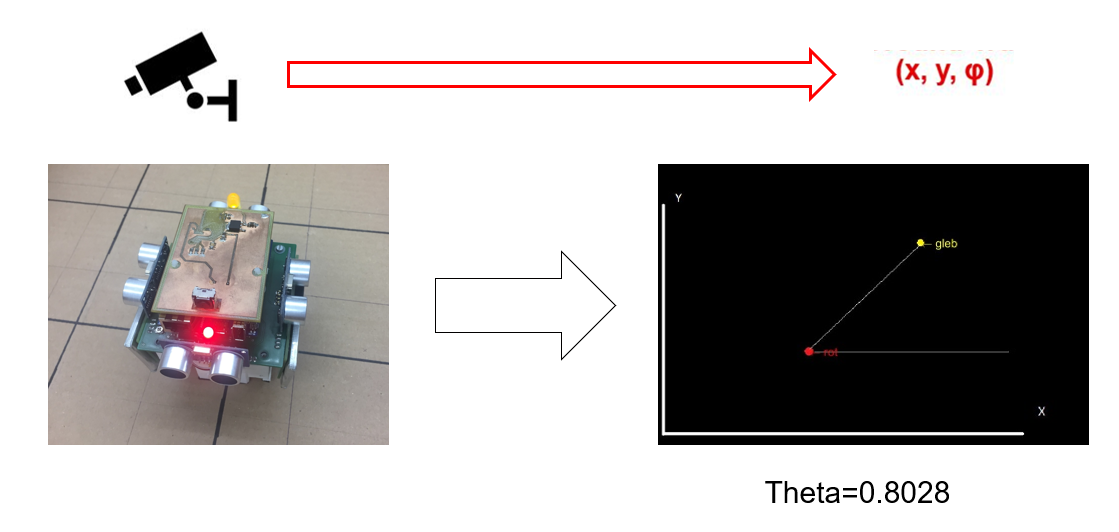
\includegraphics[width=0.9\linewidth]{Images/camera.png}
	\caption{Erkennung der LEDs aus dem Kamerabild, zum Tracking des Laufroboters.}
	\label{fig:crawler}
\end{figure}

\begin{figure}
	\centering
	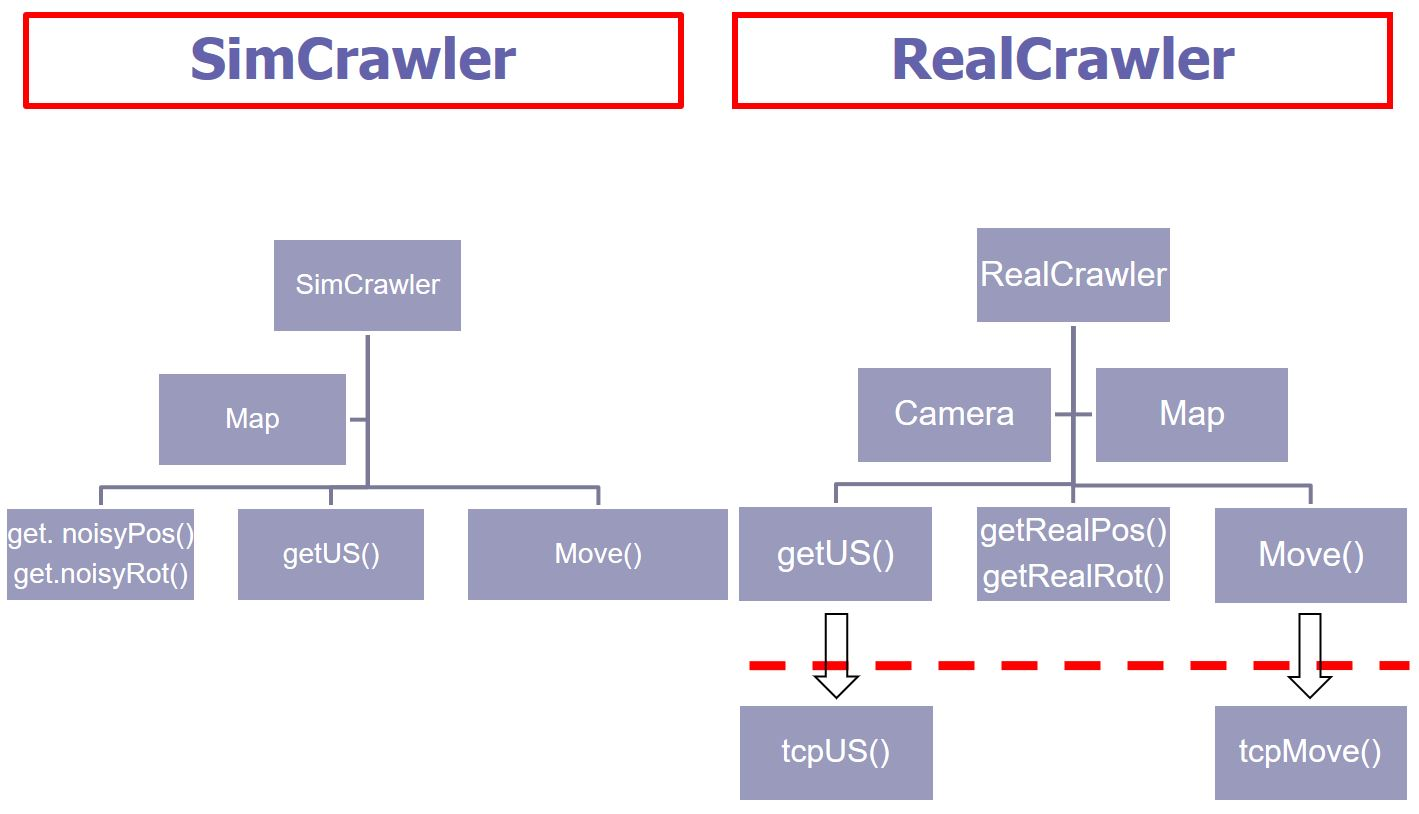
\includegraphics[width=0.9\linewidth]{Images/crawlerklass.jpg}
	\caption{Gemeinsam genutzte Schnittstelle der Crawler-Klassen}
	\label{fig:crawler}
\end{figure}
\clearpage
